\documentclass[10pt]{article}
\usepackage[a4paper,margin=1.55cm]{geometry}
\usepackage{booktabs,longtable,array,graphicx,xcolor,caption,amsmath,multirow}
\graphicspath{{image/}}
\newcolumntype{L}[1]{>{\raggedright\arraybackslash}p{#1}}
\setlength{\parindent}{0pt}
\setlength{\parskip}{4pt}
\captionsetup{font=small}

\begin{document}
\begin{center}
{\Large\bfseries Supplementary Material}\\[3pt]
{\large LitePhish: Resource-Efficient URL-Intrinsic Phishing Detection for Consumer Electronics}
\end{center}

\color{black}

\section{URL-Intrinsic Feature Representation}

LitePhish derives all inference variables from the observed URL string. It does not retrieve webpage content, resolve redirect chains, query domain-registration records, or use online reputation services. The representation combines 86 handcrafted lexical, structural, compositional, transition, heuristic, and entropy descriptors with character 2-grams and 3-grams. The handcrafted descriptors summarize interpretable URL morphology, whereas the N-gram representation captures short local sequences that aggregate descriptors may not express. These variables are statistical indicators rather than causal evidence of maliciousness; their interpretation depends on the training distribution and the surrounding feature context.

Table~\ref{tab:features} defines the 86 handcrafted descriptors. Ratio denominators are protected against division by zero. Entropy variables use Shannon entropy on the indicated character sequence, and Boolean indicators take values in $\{0,1\}$. Terms such as ``suspicious'' or ``risk'' denote fixed URL-intrinsic lexical rules; they do not imply an external reputation lookup.

\small
\begin{longtable}{r L{3.4cm} L{5.1cm} L{6.0cm}}
\caption{Handcrafted URL-intrinsic descriptors. Security interpretations are hypotheses motivating inclusion, not deterministic rules.}\label{tab:features}\\
\toprule
\textbf{No.} & \textbf{Feature} & \textbf{Definition} & \textbf{Security interpretation} \\
\midrule
\endfirsthead
\toprule
\textbf{No.} & \textbf{Feature} & \textbf{Definition} & \textbf{Security interpretation} \\
\midrule
\endhead
1 & URL length & Total URL character count & Long strings may conceal salient tokens in paths or queries. \\
2 & Hostname length & Hostname character count & Unusually long hostnames may reflect deceptive or generated naming. \\
3 & Domain length & Registrable-domain label length & Long core labels may occur in squatting or generated domains. \\
4 & TLD length & Top-level-domain length & Captures variation in suffix morphology. \\
5 & Subdomain length & Combined subdomain character count & Long subdomains may place trusted terms outside the registrable domain. \\
6 & Path length & URL-path character count & Long paths may contain nested or encoded material. \\
7 & Query-string length & Query character count & Parameter-heavy URLs may conceal redirection or tracking values. \\
8 & Maximum token length & Longest delimiter-separated token & Very long tokens may indicate encoded or generated strings. \\
9 & Minimum token length & Shortest nonempty token & Captures tokenization structure. \\
10 & Mean token length & Mean nonempty-token length & Summarizes lexical granularity. \\
11 & Digit count & Number of digits in the URL & Digit density may reflect identifiers, IP-like forms, or generated strings. \\
12 & Subdomain depth & Number of subdomain labels & Deep host hierarchies may support visual deception. \\
13 & Domain hierarchy depth & Number of hostname labels & Captures hostname structural complexity. \\
14 & TLD structure depth & Number of public-suffix components & Distinguishes single- and multipart public suffixes. \\
15 & Encoded-hostname indicators & Count of nonalphanumeric hostname characters & Captures hostname punctuation. \\
16 & Slash count & Number of slash characters & Approximates path and scheme structure. \\
17 & Dot count & Number of dot characters & Reflects host depth and IP-like notation. \\
18 & Hostname hyphen count & Number of hyphens in the hostname & Hyphens may separate impersonation tokens. \\
19 & Query-parameter count & Number of ampersand-delimited query fields & Captures query complexity. \\
20 & Path depth & Number of slash characters in the parsed path & Captures hierarchical depth. \\
21 & Port number & Parsed explicit port, if present & Represents nondefault service addressing. \\
22 & Has port & Indicator of explicit port presence & Flags nondefault URL authority syntax. \\
23 & Path-traversal depth & Count of parent-directory tokens & Represents traversal-like lexical patterns. \\
24 & Domain-to-URL ratio & Domain length divided by URL length & Distinguishes host-dominant and path-dominant strings. \\
25 & Subdomain-to-URL ratio & Subdomain length divided by URL length & Quantifies subdomain prominence. \\
26 & Hostname-to-URL ratio & Hostname length divided by URL length & Quantifies authority prominence. \\
27 & Path-to-URL ratio & Path length divided by URL length & Quantifies path prominence. \\
28 & Query-to-URL ratio & Query length divided by URL length & Quantifies query prominence. \\
29 & Path-to-domain ratio & Path length divided by domain length & Measures path complexity relative to the core domain. \\
30 & Query-to-domain ratio & Query length divided by domain length & Measures query complexity relative to the core domain. \\
31 & Query-to-path ratio & Query length divided by path length & Characterizes query--path balance. \\
32 & Uppercase ratio & Number of uppercase URL characters divided by URL length & Captures case variation that may fragment lexical patterns. \\
33 & Subdomain digit ratio & Fraction of regex tokens $[a$--$z]^+$ or $\backslash d^+$ that are wholly numeric & Quantifies numeric subdomain tokens. \\
34 & Hostname entropy & Shannon entropy of hostname characters & Captures hostname randomness. \\
35 & Path entropy & Shannon entropy of path characters & Captures opaque path material. \\
36 & Query entropy & Shannon entropy of query characters & Captures opaque parameter material. \\
37 & URL 2-gram entropy & Shannon entropy of overlapping URL character pairs & Quantifies pairwise sequence diversity. \\
38 & URL 3-gram entropy & Shannon entropy of overlapping URL character triples & Quantifies triplet diversity. \\
39 & Hostname 2-gram entropy & Shannon entropy of overlapping hostname pairs & Quantifies local hostname diversity. \\
40 & Domain entropy & Shannon entropy of registrable-domain characters & Captures core-domain randomness. \\
41 & Path-entropy variance & Variance of Shannon entropy across nonempty path segments; zero for fewer than two & Detects localized path irregularity. \\
42 & Rolling-entropy range & Maximum minus minimum entropy across overlapping five-character URL windows & Captures within-URL changes in randomness. \\
43 & Subdomain-entropy gradient & Entropy of the first subdomain label minus that of the last; zero for fewer than two labels & Captures heterogeneous hostname composition. \\
44 & Cookie-parameter entropy & Entropy of concatenated values for sessionid, sessid, sid, token, auth, uid, user\_id, and cookie keys & Represents opaque session-related values. \\
45 & Digits in hostname & Number of hostname digits & Captures numeric host morphology. \\
46 & Alphabetic in hostname & Number of alphabetic hostname characters & Complements numeric and punctuation counts. \\
47 & Punctuation in URL & Count of characters in !@\#\$\%\^\&*() & Summarizes selected punctuation. \\
48 & Non-ASCII in URL & Count of URL characters with code point greater than 127 & Captures Unicode forms. \\
49 & Alpha ratio in hostname & Alphabetic hostname characters divided by hostname length & Characterizes alphabetic composition. \\
50 & Digit ratio in hostname & Hostname digits divided by hostname length & Characterizes numeric composition. \\
51 & Special-character ratio in hostname & Nonalphanumeric hostname characters divided by hostname length & Characterizes unusual punctuation. \\
52 & Homoglyph score & Count of Cyrillic characters corresponding visually to Latin a, e, i, o, and c in the hostname & Represents the fixed five-character confusable set. \\
53 & Letter--digit--letter count & Count of positions whose center is a digit flanked by letters & Captures mixed-character patterns. \\
54 & Digit--letter--digit count & Count of positions whose center is a letter flanked by digits & Captures mixed-character patterns. \\
55 & Alpha--digit transitions & Adjacent letter-to-digit transitions divided by URL length & Quantifies character-type switching. \\
56 & Digit--alpha transitions & Adjacent digit-to-letter transitions divided by URL length & Quantifies character-type switching. \\
57 & Consecutive characters & Number of adjacent identical-character pairs & Captures repetition. \\
58 & Consecutive digits & Number of adjacent digit--digit pairs & Captures numeric runs. \\
59 & Consecutive letters & Number of adjacent letter--letter pairs & Captures alphabetic runs. \\
60 & Special-character cluster & Maximum length of a run of at least two characters outside $\backslash w$, dot, slash, and hyphen & Captures localized symbol concentration. \\
61 & Pattern density & Mean distinct-character count across overlapping five-character URL windows & Summarizes local diversity. \\
62 & Suspicious keyword & Indicator that the lowercased URL contains a term from the released fixed lexicon & Represents lure and account-action terminology. \\
63 & URL shortener & Indicator for bit.ly, goo.gl, tinyurl.com, t.co, is.gd, buff.ly, adf.ly, or bc.vc; also flags dotless hostnames of length at most five & Represents hidden destinations without resolving redirects. \\
64 & Digits in subdomain & Indicator that any subdomain character is numeric & Captures identifier-bearing subdomains. \\
65 & Redirect in path & Indicator that the parsed path contains // or the token redirect & Represents redirection morphology. \\
66 & Long numeric domain & Indicator that the registrable domain exceeds eight characters and contains a digit & Captures generated-looking domains. \\
67 & TLD risk score & 0 for domains containing a released legitimate/trust lexicon term; otherwise 1 for a suspicious-domain term, 0.9 for a released rare suffix, and 0 otherwise & Fixed lexical rule without online lookup. \\
68 & Suspicious hosting & Indicator that the hostname contains a term from the released suspicious-domain lexicon & Represents shared-hosting patterns. \\
69 & Numeric domain pattern & Indicator that domain digit ratio exceeds 0.3 or digit count exceeds three & Captures numeric domain morphology. \\
70 & Hex-encoded IP & Indicator matching either hexadecimal 0x plus eight hexadecimal digits or dotted-decimal notation & Captures noncanonical address forms. \\
71 & TLD--domain mismatch & Indicator that domain length lies outside com 3--12, net 3--10, org 3--8, or io 2--6; other suffixes are flagged & Encodes a fixed suffix-specific rule. \\
72 & Port mismatch & Indicator that an explicit port is outside \{80,443,8080,8000,3000\} & Represents nonstandard service addressing. \\
73 & IP as hostname & Indicator for exactly four decimal octets in $[0,255]$ & Distinguishes literal IPv4 hosts. \\
74 & Non-HTTP scheme & Zero only when the parsed scheme is http; one otherwise & Encodes the fixed scheme rule. \\
75 & WWW prefix & Indicator that the hostname begins with www. & Represents a common hostname convention. \\
76 & TLD is .com & Indicator that the extracted suffix equals com & Represents a frequent suffix. \\
77 & Punycode domain & Indicator that the registrable-domain label begins with xn-- & Captures internationalized-domain encoding. \\
78 & URL character diversity & Unique URL characters divided by URL length & Summarizes alphabet diversity. \\
79 & Hostname character diversity & Unique hostname characters divided by hostname length & Summarizes host diversity. \\
80 & Obfuscation characters & Indicator for a percent sign or any non-ASCII URL character & Captures encoded or internationalized notation. \\
81 & Encoding keywords & Indicator matching base64 or hex followed by a nonalphanumeric character & Captures explicit encoding terminology. \\
82 & Redirect keywords & Indicator that a nonempty query contains redirect, url=, or goto= & Captures query-mediated redirection cues. \\
83 & Redirect-chain count & Count of // minus the scheme delimiter when :// is present & Counts visible redirect-like delimiters. \\
84 & Consecutive special characters & Number of adjacent identical nonalphanumeric pairs & Captures repeated punctuation. \\
85 & Encoding-bypass ratio & Count of percent escapes other than \%20, \%21, \%2F, \%3A, \%3F, and \%3D divided by URL length & Quantifies uncommon percent encoding. \\
86 & Redirect-TLD disparity & Indicator that an embedded URL under redirect, url, return, goto, or dest has a suffix different from the outer URL & Represents visible cross-domain redirection. \\
\bottomrule
\end{longtable}
\normalsize


\section{Training-Only Parameter Selection}

All representation fitting uses the source training partition, while hyperparameter selection uses only the source training and validation partitions. Validation phishing-class F1 selects $(\gamma,\alpha)=(0.55,0.90)$ for PhishStorm-source transfer and $(0.55,0.95)$ for the primary PhishFusion model; the Ebbu2017-source setting is $(0.30,0.95)$. Target-dataset labels are not used for feature selection, model selection, or fitting. The PhishFusion primary model uses 568 selected features; source-specific cross-dataset models retain 939 features for PhishStorm and 821 for Ebbu2017.

Character 2-/3-gram selection uses $df_{\min}=5$, $df_{\max}=1.0$, variance threshold $\tau=10^{-5}$, composite weight $\beta=0.5$, and $K_{\mathrm{ng}}=5{,}000$. SDCS uses $S=20$ subsamples, a subsampling fraction of 0.905, L1-logistic inverse-regularization $C=0.191$, $\tau_{\mathrm{stab}}=0.705$, $w_m=0.318$, $w_s=0.767$, $\rho_{\max}=0.956$, and $K=1{,}000$. Mutual information is estimated from at most 20,000 source-training observations.

\section{Detailed Ablation Results}

\subsection{Complete SDCS procedure}

Given the training-only feature pool $F_{\mathrm{all}}$, labels $Y$, stability iterations $S$, regularization $\lambda$, stability threshold $\tau_{\mathrm{stab}}$, weights $(w_m,w_s)$, redundancy threshold $\rho_{\max}$, and selection limit $K$, SDCS performs the following operations:
\begin{enumerate}
\item Draw $S$ randomized training subsamples, fit L1-regularized logistic regression to each, and compute the nonzero-coefficient selection frequency $\operatorname{Stab}(f)$ for every feature.
\item Retain $F_{\mathrm{stable}}=\{f:\operatorname{Stab}(f)\geq\tau_{\mathrm{stab}}\}$.
\item Compute normalized mutual information and XGBoost gain on $F_{\mathrm{stable}}$, and combine them as $\operatorname{HIScore}(f)=w_m\operatorname{Imp}_{\mathrm{mi}}(f)+(1-w_m)\operatorname{Imp}_{\mathrm{gbt}}(f)$.
\item Rank features by $C(f)=w_s\operatorname{Stab}(f)+(1-w_s)\operatorname{HIScore}(f)$.
\item Traverse the ranking and retain a feature only when its absolute Pearson correlation with every previously retained feature is below $\rho_{\max}$; stop when $K$ features have been retained or the ranking is exhausted.
\end{enumerate}

\begin{table}[ht]
\centering
\caption{Handcrafted-feature ablation on PhishFusion. Metrics are percentages.}
\begin{tabular}{lrrrrrrr}
\toprule
Configuration & Acc. & Prec. & Rec. & F1 & AUC & Features & Reduction \\
\midrule
FL-LGBM, full $F_{\mathrm{hc}}$ & 93.40 & 98.13 & 89.84 & 93.80 & 99.32 & 86 & -- \\
Standard LGBM, full $F_{\mathrm{hc}}$ & 87.96 & 98.93 & 79.20 & 87.97 & 99.27 & 86 & -- \\
FL-LGBM, $F_{\mathrm{hc}}$+SDCS & 94.62 & 98.03 & 92.18 & 95.02 & 99.34 & 62 & 28\% \\
Standard LGBM, $F_{\mathrm{hc}}$+SDCS & 89.28 & 98.54 & 79.90 & 88.24 & 99.11 & 62 & 28\% \\
\bottomrule
\end{tabular}
\end{table}

\begin{table}[ht]
\centering
\caption{Component-level SDCS ablation on PhishFusion. Metrics are percentages.}
\label{tab:sdcs_component}
\begin{tabular}{lrrrrr}
\toprule
Variant & Acc. & Prec. & Rec. & F1 & AUC \\
\midrule
MI only & 96.42 & 97.36 & 96.11 & 96.72 & 99.52 \\
Gain only & 96.70 & 97.51 & 96.40 & 96.96 & 99.57 \\
Stability only & 96.25 & 97.08 & 96.04 & 96.56 & 99.46 \\
MI + gain & 96.95 & 97.73 & 96.72 & 97.22 & 99.65 \\
SDCS without correlation pruning & 97.20 & 97.91 & 96.98 & 97.44 & 99.70 \\
Full SDCS & 97.51 & 98.11 & 97.33 & 97.72 & 99.75 \\
\bottomrule
\end{tabular}
\end{table}

For the seed-42 PhishFusion paired analysis, the raw 56,601-feature representation and the 568-feature compact representation were evaluated under an identical one-core/512~MiB protocol. Table~\ref{tab:compact} separates the effects of feature selection on predictive performance, fitting time, storage, memory, and inference latency.

{
The component ablation in Table~\ref{tab:sdcs_component} yields 97.51\% accuracy and 97.72\% F1 for Full SDCS. A fixed-seed paired experiment evaluates representation compactness using seed 42, identical domain-disjoint partitions, focal parameters, and LightGBM hyperparameters for the raw and compact models. Selection increases accuracy from 97.47\% to 97.72\%, recall from 96.73\% to 97.45\%, F1-score from 97.70\% to 97.94\%, and ROC-AUC from 99.73\% to 99.77\%, while precision changes from 98.69\% to 98.44\%. Model-fitting time decreases from 70.31 to 15.43~s, a 78.1\% reduction (4.56$\times$). The component ablation evaluates the SDCS stages, whereas the paired experiment evaluates reduction of the complete representation.
}

\begin{table}[ht]
\centering
\caption{{Direct resource and model-fitting comparison of raw and compact LitePhish representations. FE denotes URL-to-feature extraction; Total includes FE, preprocessing, and prediction. Inference values are medians over four independent profiling passes.}}
\label{tab:compact}
\small
\resizebox{\textwidth}{!}{\begin{tabular}{llrrrrrrr}
\toprule
Representation & Profile & Features & Bundle (MB) & {Fit (s)} & Peak RSS (MiB) & {FE (ms/URL)} & Total (ms/URL) & URL/s \\
\midrule
Raw & Online & 56,601 & 4.385 & {70.31} & 232.76 & {1.233} & 3.188 & 313.7 \\
Raw & Batched & 56,601 & 4.385 & {--} & 232.36 & {0.944} & 1.001 & 999.4 \\
Compact & Online & 568 & 1.874 & {15.43} & 227.25 & {2.129} & 3.805 & 262.8 \\
Compact & Batched & 568 & 1.874 & {--} & 227.67 & {0.933} & 1.008 & 991.9 \\
\bottomrule
\end{tabular}}
\end{table}

{Resource values in Table~\ref{tab:compact} are medians across four profiling passes for the raw and compact models. The five-model benchmark in the main article reports means across three passes. Because the model representations, timing boundaries, and aggregation differ, the values are compared within each protocol.}

\section{Imbalance-Objective Analysis}

PhishFusion training subsets were constructed at phishing-to-benign ratios of 1:3, 1:5, and 1:10. The primary analysis compares focal, standard, and class-weighted LightGBM across ten paired seeds using a common decision threshold of 0.5. A secondary sensitivity analysis compares focal and standard LightGBM after selecting the decision threshold by validation F1 within each seed. Table~\ref{tab:focal} reports focal-minus-baseline F1 differences. Confidence intervals are paired Student-$t$ intervals; inference also includes paired $t$ and Wilcoxon tests with Holm correction. Because normality is uncertain in several ten-seed contrasts, the interpretation emphasizes agreement between effect intervals and adjusted rank-based tests.

\begin{table}[ht]
\centering
\caption{Paired F1 comparison of focal weighting. ``Fixed'' uses a common threshold of 0.5; ``validation-selected'' chooses the threshold by validation F1 within each seed.}
\label{tab:focal}
\begin{tabular}{llllrrr}
\toprule
Ratio & Threshold & Baseline & Focal F1 & Baseline F1 & Difference (95\% CI) & Holm Wilcoxon $p$ \\
\midrule
1:3 & Fixed & Standard & .957 & .886 & .071 (.060,.082) & .0234 \\
1:3 & Fixed & Class weighted & .957 & .894 & .064 (.050,.077) & .0234 \\
1:5 & Fixed & Standard & .928 & .875 & .053 (.038,.068) & .0234 \\
1:5 & Fixed & Class weighted & .928 & .892 & .036 (.018,.054) & .0313 \\
1:10 & Fixed & Standard & .894 & .853 & .041 (.017,.066) & .0234 \\
1:10 & Fixed & Class weighted & .894 & .872 & .022 ($<$.001,.045) & .1914 \\
1:3 & Validation-selected & Standard & .966 & .946 & .020 (.002,.038) & .2227 \\
1:5 & Validation-selected & Standard & .964 & .960 & .003 (-.007,.014) & 1.000 \\
1:10 & Validation-selected & Standard & .953 & .964 & -.011 (-.031,.009) & 1.000 \\
\bottomrule
\end{tabular}
\end{table}

\section{Temporal and Failure-Case Evaluation}

The prospective temporal cohort contains 290 confirmed OpenPhish URLs collected after the training cutoff. Because it contains no benign examples, only recall and score distributions are identifiable. LitePhish detects 256 URLs and misses 34, giving 88.28\% recall (Wilson 95\% CI: 84.06--91.49\%). The mean and median phishing probabilities are 0.868 and 0.996, respectively. The {time-indexed PhishFusion model} obtains 97.45\% recall on its internal positive test subset, which provides the in-distribution reference. {Failure-stratum and counterfactual analyses use a separate seed-42 domain-disjoint model with 96.76\% phishing recall; each reference value is therefore interpreted within its own analysis.}

\begin{table}[ht]
\centering
\caption{Natural error strata on the PhishFusion test partition. Categories are rule-defined and mutually assigned for analysis.}
\begin{tabular}{llrrr}
\toprule
Category & Class & $n$ & Errors & Error rate (Wilson 95\% CI) \\
\midrule
All & Phishing & 6,325 & 205 & .0324 (.0283,.0371) \\
All & Benign & 5,051 & 90 & .0178 (.0145,.0218) \\
Shared/reputable host & Phishing & 554 & 120 & .2166 (.1843,.2528) \\
Clean-looking & Phishing & 649 & 13 & .0200 (.0117,.0340) \\
Obfuscated & Phishing & 3,671 & 52 & .0142 (.0108,.0185) \\
Obfuscated & Benign & 55 & 13 & .2364 (.1437,.3635) \\
Clean-looking & Benign & 817 & 54 & .0661 (.0510,.0852) \\
\bottomrule
\end{tabular}
\end{table}

Counterfactual transformations probe sensitivity while preserving the original labels. A shortening-service proxy reduces recall from 0.9676 to 0.5535; clean-surface transformation reduces it to 0.7968; a reputable-host proxy reduces it to 0.9492; masking brand tokens in 1,035 applicable URLs reduces recall from 0.8850 to 0.8725. Separator obfuscation leaves recall unchanged within its paired interval, whereas percent-encoding the path slightly increases recall. These transformations do not resolve live redirects or establish the behavior of a complete browser navigation chain; they isolate lexical sensitivity.

The popular-DNS stress cohort retains 89,937 names from the top 100,000 Umbrella ranks after exclusion of effective domains associated with known phishing samples. These are popularity-based likely-benign proxies rather than individually verified benign browser visits. At threshold 0.5, 74,175 names are labeled phishing, giving an 82.47\% false-positive rate (Wilson 95\% CI: 82.22--82.72\%). This rate indicates that bare DNS-name inputs require deployment-specific normalization and threshold validation.

\section{Resource and Energy Measurement}

The common latency protocol evaluates Ebbu, E2Phish, MUDS, TabNet, and LitePhish sequentially on identical fixed-seed URL cohorts, including each model's feature construction. A Linux cgroup enforces one CPU core and 512~MiB RAM on an Intel Xeon Gold 6240 host. Online measurements use batch size 1; batch measurements use 100 URLs. Warm-up observations are excluded. Peak resident memory includes the process and its descendants.

CPU-package energy is measured independently on an Intel Core i7-9700 desktop. Each model is pinned to one core and processes 5,000 unique URLs in batches of 100 for five randomized trials. Two warm-up passes are excluded. Each active phase lasts at least 33.6~s and contains at least 149 hardware-monitor samples; an adjacent 10~s idle phase provides the baseline subtraction. The resulting values exclude display, network, storage, power-supply losses, and other system components and therefore quantify CPU-package rather than whole-device energy.

\begin{table}[ht]
\centering
\caption{Idle-adjusted CPU-package energy. Confidence intervals use Student's $t$ distribution with four degrees of freedom.}
\begin{tabular}{lrrr}
\toprule
Model & mJ/URL (mean) & 95\% CI & URLs/J \\
\midrule
MUDS & 2.415 & 2.083--2.747 & 414.12 \\
LitePhish & 7.022 & 6.317--7.726 & 142.41 \\
E2Phish & 45.289 & 30.975--59.603 & 22.08 \\
TabNet & 89.460 & 55.433--123.487 & 11.18 \\
Ebbu & 341.097 & 265.986--416.209 & 2.93 \\
\bottomrule
\end{tabular}
\end{table}

MUDS is 2.91 times more energy efficient than LitePhish and also has the smallest inference bundle. LitePhish attains higher phishing-class F1 under domain-stratified, cross-dataset, and external evaluations. Relative to E2Phish, TabNet, and Ebbu, LitePhish reduces CPU-package energy per URL by 84.5\%, 92.2\%, and 97.9\%, respectively. These findings characterize a multi-objective accuracy--storage--latency--energy trade-off.

\section{Paired Statistical Comparisons}

Prediction-level comparisons span the three internal domain-disjoint datasets, four cross-dataset transfers, and the external cohort. Accuracy differences use exact McNemar tests and paired multinomial-bootstrap intervals; phishing-class F1 uses paired multinomial bootstrap; ROC-AUC uses paired DeLong tests. Holm correction is applied within each table and metric family, yielding 72 LitePhish--baseline comparisons. On the external {93,788-URL cohort (42,335 phishing and 51,453 benign)}, LitePhish exceeds all nine baselines in accuracy, phishing-class F1, and ROC-AUC after Holm correction. {The direction and significance of differences vary across individual metrics and source--target settings. LitePhish obtains the highest phishing-class F1 in all four transfers, whereas DEPHIDES and URLNet obtain the highest ROC-AUC in the two Ebbu2017-source transfers; the interpretation therefore distinguishes F1 performance from ranking performance.}

\section{Merged-Corpus Keyword Analysis}

The merged descriptive corpus combines PhishFusion, Ebbu2017, and PhishStorm for an aggregate analysis of URL-token distributions. It contains 126,387 phishing URLs and 130,899 benign URLs, spanning 44,389 and 31,746 unique root domains, respectively. Table~\ref{tab:merged_interpretability} summarizes its composition.

\begin{table}[ht]
\centering
\caption{Composition of the merged corpus used for keyword-frequency analysis.}
\label{tab:merged_interpretability}
\small
\begin{tabular}{llrrrr}
\toprule
Dataset & Label & URLs & Root domains & With path & With query \\
\midrule
Merged & Phishing & 126,387 & 44,389 & 120,855 & 33,258 \\
       & Benign   & 130,899 & 31,746 & 129,242 & 6,245 \\
\bottomrule
\end{tabular}
\end{table}

Figure~\ref{fig:merged_landscape} summarizes frequent lexical and domain-related tokens in the phishing subset. The lexical view contains file extensions, hosting terms, authentication-related expressions, and brand-associated terms. The domain view contains public suffixes and hosting-domain fragments. These visualizations characterize the observed corpus composition and are not domain-reputation scores.

\begin{figure}[ht]
\centering
\begin{minipage}[t]{0.49\textwidth}
\centering
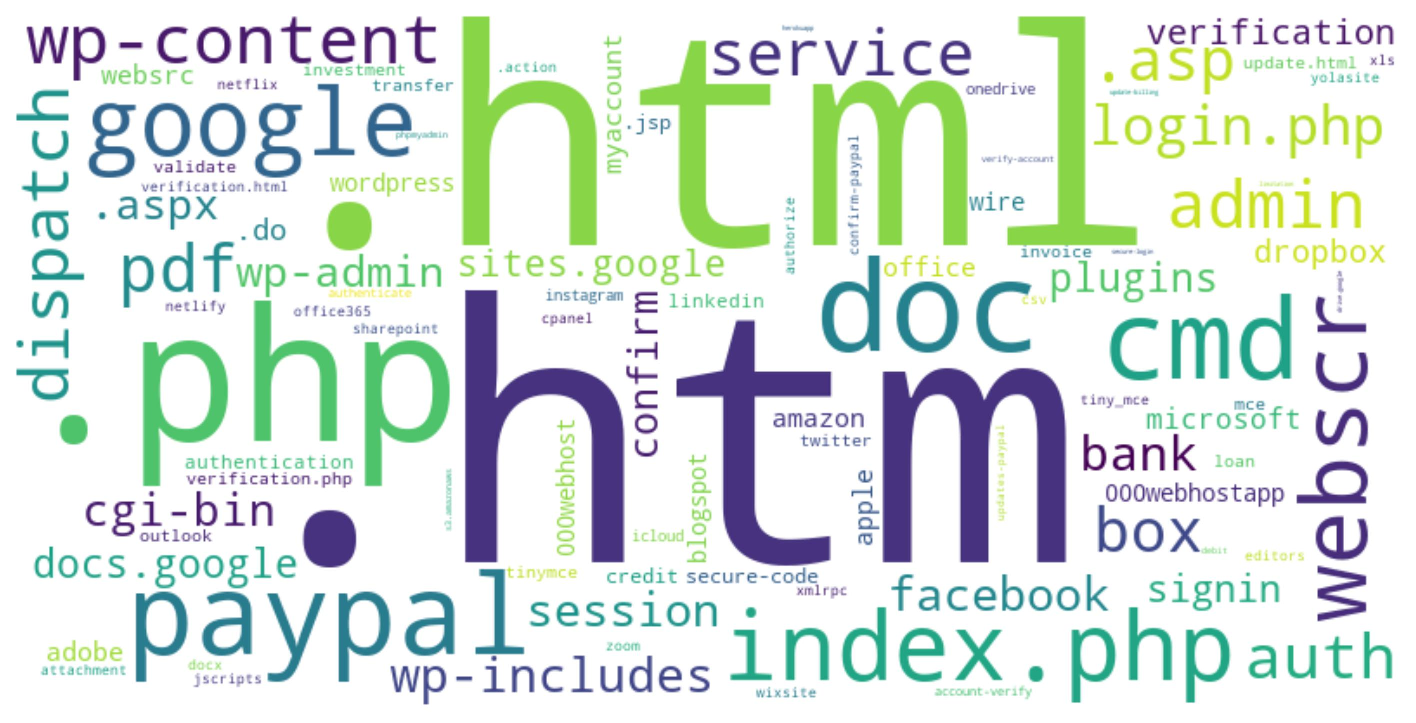
\includegraphics[width=\linewidth]{Merged_Suspicious_Terms}
\\[-2pt]\small (a) Frequent lexical tokens
\end{minipage}\hfill
\begin{minipage}[t]{0.49\textwidth}
\centering
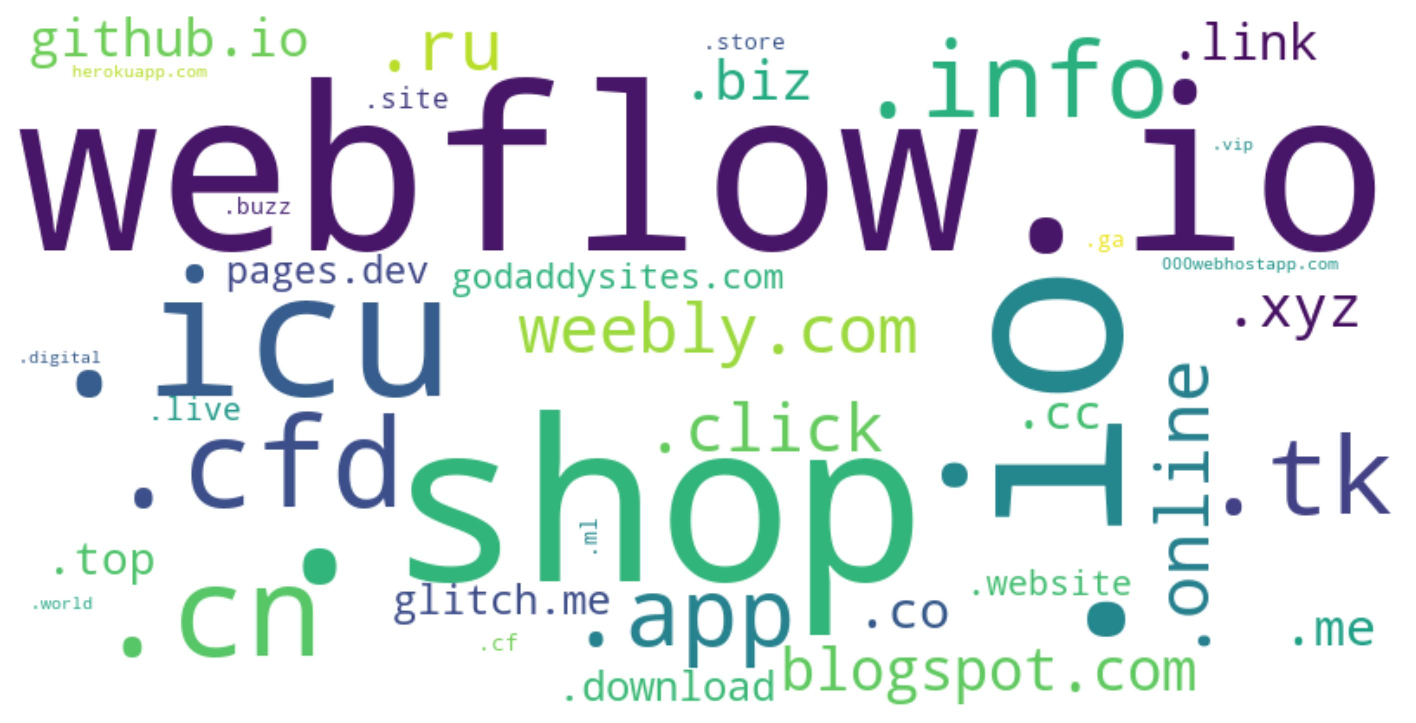
\includegraphics[width=\linewidth]{Merged_Domain_Suffix_Tokens}
\\[-2pt]\small (b) Frequent domain and suffix tokens
\end{minipage}
\caption{Descriptive token landscape of phishing URLs in the merged corpus. Text size represents relative occurrence frequency within each visualization.}
\label{fig:merged_landscape}
\end{figure}

Figure~\ref{fig:merged_keywords} compares class-conditional occurrence counts for prominent URL tokens. Technical suffixes such as \texttt{.html} and \texttt{.htm} occur frequently in both classes, whereas \texttt{.php} and several impersonation-related tokens, including \texttt{paypal}, \texttt{google}, and \texttt{secure}, show substantially higher counts in the phishing subset. The class contrast provides corpus-level context for the model-based SHAP findings, without treating any single token as sufficient evidence of phishing.

\begin{center}
\centering
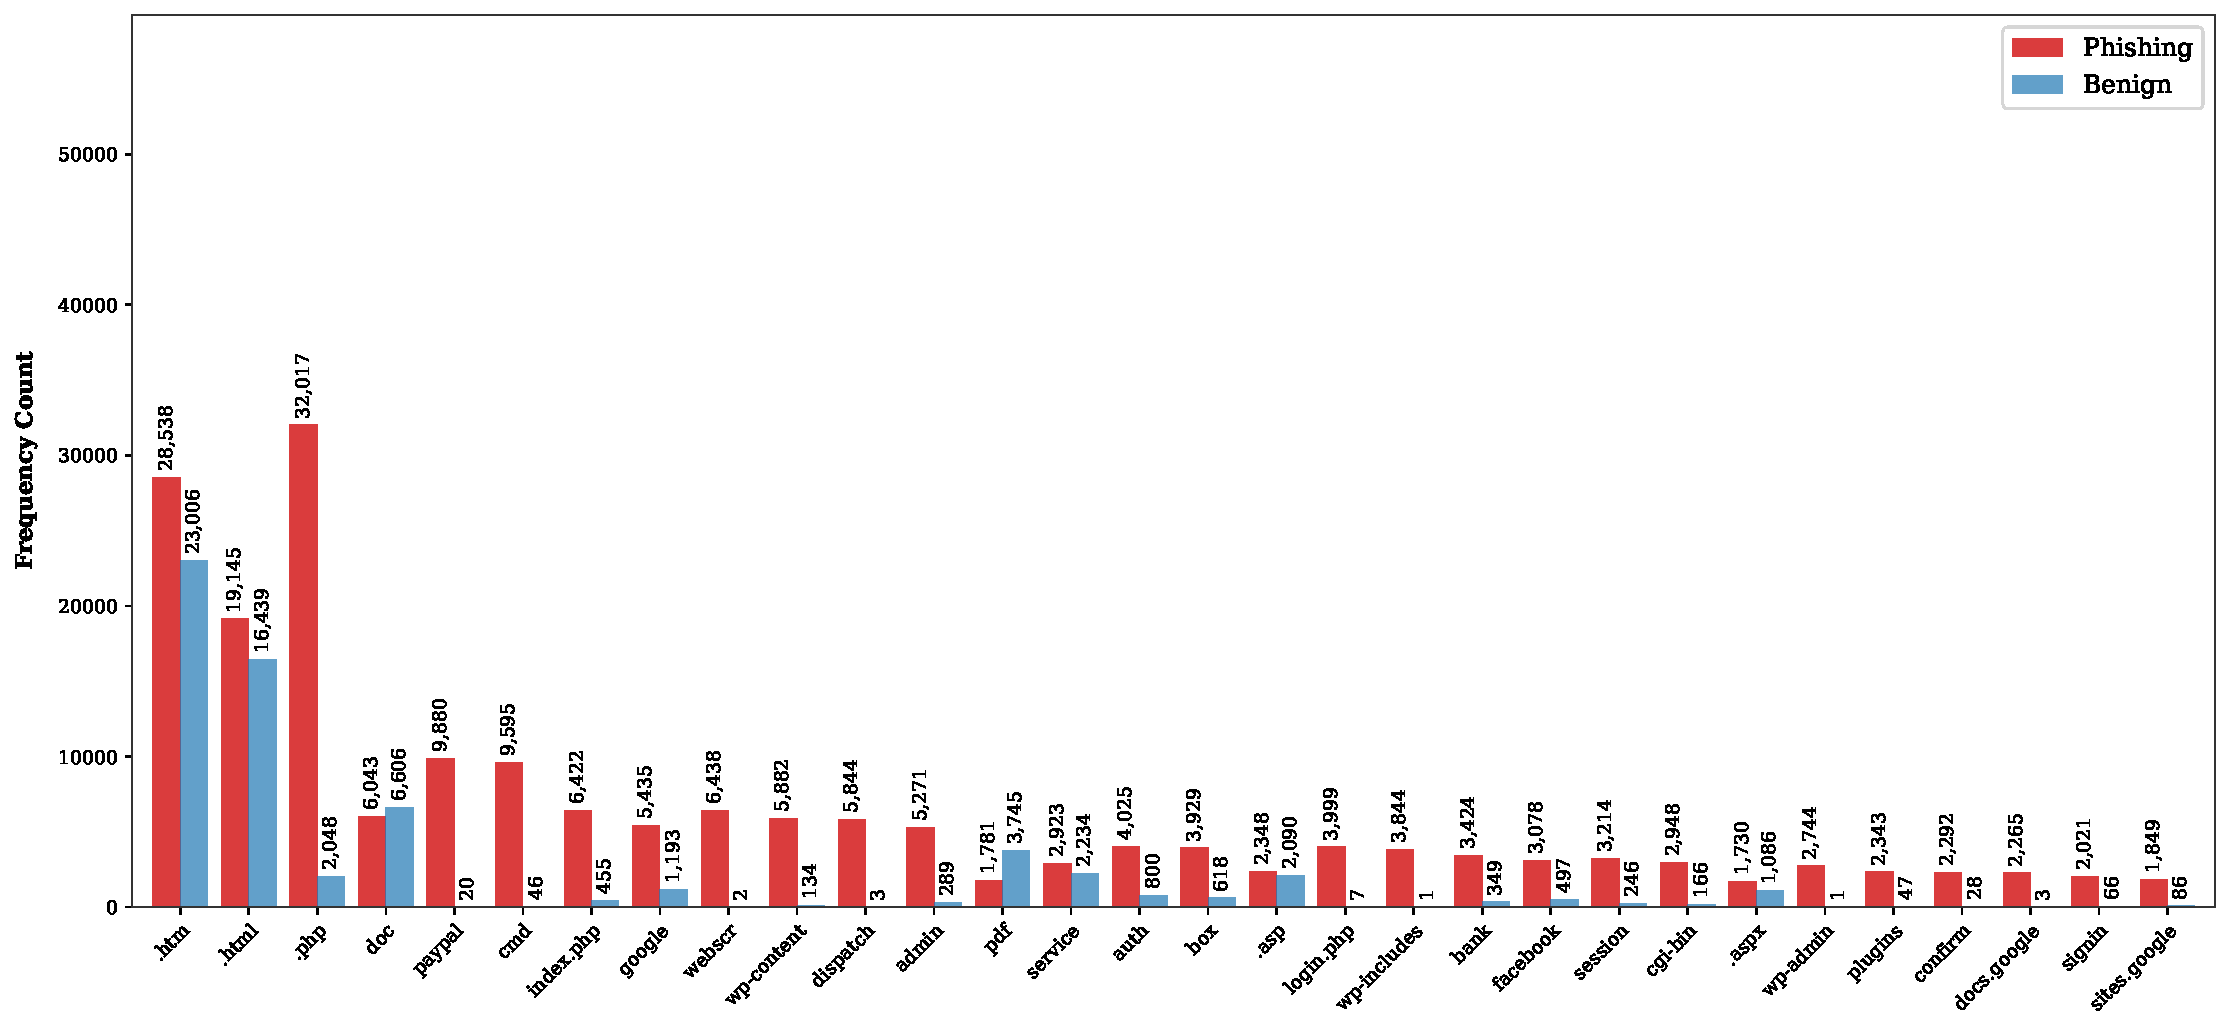
\includegraphics[width=0.90\textwidth]{Merged_Token_Frequencies}
\captionof{figure}{Class-conditional occurrence counts of prominent URL tokens in the merged corpus. Counts may reflect source composition, repeated campaigns, hosting infrastructure, and collection period.}
\label{fig:merged_keywords}
\end{center}

\section{Interpretability Scope}

The keyword-frequency, suffix, and SHAP summaries characterize associations within the observed data. They do not establish causal effects or guarantee that a token will retain the same direction under distribution shift. In particular, brand terms, shared-hosting patterns, and technical suffixes also occur in benign URLs. The high false-positive rate on the popular-DNS proxy and the counterfactual host transformations demonstrate why these features must be interpreted jointly rather than as deterministic indicators.

\section{Scope and Limitations of Resource Measurements}

{The study measures inference-bundle size, feature-construction cost, latency, peak RAM, constrained one-core execution, and CPU-package energy. These quantities characterize computational feasibility on the evaluated x86-64 systems. No physical Raspberry Pi, smartphone, ARM gateway, or microcontroller is evaluated; architecture-specific latency, thermal behavior, battery consumption, and whole-device energy therefore remain unquantified. Device-level performance requires direct measurement on the intended hardware.}

\end{document}
